\documentclass[a4paper,12pt,notitlepage]{mwrep}
%\usepackage{fullpage}

\usepackage[a4paper, margin=6em, vmargin={6em, 8em}]{geometry}
\usepackage{ltxtable}
\usepackage{verbatim}
\usepackage{float}
\usepackage{listings}
\usepackage{tabularx}
%\addtolength{\oddsidemargin}{-.25cm}
%\addtolength{\evensidemargin}{-.25cm}
%\addtolength{\textwidth}{0.5cm}
%\addtolength{\topmargin}{+.25cm}
%\addtolength{\textheight}{0.5cm}

\usepackage{fancyhdr}
\pagestyle{fancyplain}

\renewcommand{\chaptermark}[1]{\markboth{#1}{}}
% section number and title
\renewcommand{\sectionmark}[1]{\markright{\thesection\ #1}}

\usepackage{latexsym}
\usepackage[MeX]{polski}
\usepackage[utf8]{inputenc}% ew. utf8 lub cp12501
\usepackage[pdftex]{graphicx}
\usepackage{rotating}
\usepackage{setspace}
\usepackage{float}
\usepackage{lastpage}
\usepackage{subfig}

\newcommand{\dzien}{\today}

\newcommand{\wersja}{Wersja \textbf{1.0} z dnia \textbf{\dzien}}
\newcommand{\cfoottext}{Kraków, czerwiec 2012}
\renewcommand{\footrulewidth}{0.4pt}
\cfoot{\cfoottext}

\frenchspacing
\usepackage{listings}
\lstset{breaklines=true}

\usepackage{hyperref}
\usepackage{color}
\hypersetup{colorlinks=true}
\definecolor{mycol}{RGB}{4,27,77}
\hypersetup{linkcolor=mycol, urlcolor=mycol}

\date{\today}


\begin{document}
\begin{titlepage}
\begin{center}
  \resizebox{\textwidth}{!}{\mbox{AKADEMIA GÓRNICZO-HUTNICZA}}\\
  \vspace{2ex}
  \resizebox{\textwidth}{!}{\mbox{Wydział Elektrotechniki, Automatyki, Elektroniki i Informatyki}}\\
  \vspace{4ex}
  
\includegraphics[scale=0.15]{imgs/agh_crop.pdf} \\
  \vspace{4ex}
  \begin{large}KATEDRA INFORMATYKI\end{large} \\
  \vspace{8ex}
  \textbf{\begin{Huge}Przebieg projektu\\WEB Dispatch Rider\end{Huge}} \\
  \vspace{3ex}
  \textit{\begin{Large}Opis przebiegu prac nad projektem semestralnym\\ z Inżynierii Oprogramowania\end{Large}} \\

  \vfill

  \begin{Large}\wersja\end{Large}\\
\end{center}
\begin{large}
  \begin{tabularx}{\textwidth}{lXc}
    \textit{Kierunek, rok studiów} &  &  \\
    \hspace{3em}Informatyka, rok III &  & \\
    \textit{Przedmiot} &  & \\
	\multicolumn{3}{l}{\hspace{3em}Inżynieria Oprogramowania} \\
    \textit{Prowadzący przedmiot} &  & \textit{rok akademicki:} \hfill 2011/2012\\
    \hspace{3em}dr inż. Małgorzata Żabińska-Rakoczy &  & \textit{semestr:} \hfill letni \\
    \hspace{3em}dr inż. Jarosław Koźlak &  &\\
  \end{tabularx}
\end{large}

\vspace{2ex}

\noindent
\begin{Large}Zespół autorski:\end{Large}
\begin{large}
  \newlength{\tblwidth}
  \setlength{\tblwidth}{\textwidth}
  \addtolength{\tblwidth}{-3em}
  \begin{flushright}
    \begin{tabularx}{\tblwidth}{lXr}
      Szymon Kasiński &  & \\
      Dariusz Mydlarz &  & \\
    \end{tabularx}\end{flushright}
  \end{large}
  \thispagestyle{fancy}
\end{titlepage}


\onehalfspacing
\rfoot{\scriptsize{Strona: \thepage\  z\ \pageref{LastPage}}}
\cfoot{\scriptsize{\wersja}}

% komenda \tocless pozwoli na niepokazywanie elementu w spisie tresci
\newcommand{\nocontentsline}[3]{}
\newcommand{\tocless}[2]{\bgroup\let\addcontentsline=\nocontentsline#1{#2}\egroup}
\addtocounter{page}{1}

\tableofcontents

\vfill
\begin{center}
\singlespacing
\fbox{\begin{minipage}{0.8\textwidth}
\footnotesize Niniejsze opracowanie powstało w trakcie i jako rezultat zajęć dydaktycznych z przedmiotu 
wymienionego na stronie tytułowej, prowadzonych w Akademii Górniczo-Hutniczej w Krakowie
(AGH) przez osobę (osoby) wymienioną (wymienione) po słowach "Prowadzący zajęcia"
i nie może być wykorzystywane w jakikolwiek sposób i do jakichkolwiek celów, 
w całości lub części, w szczególności publikowane w jakikolwiek sposób
i w jakiejkolwiek formie, bez uzyskania uprzedniej, pisemnej zgody tej
osoby (tych osób) lub odpowiednich władz AGH.
\vspace{2ex} \\
\textbf{Copyright \textcopyright 2012 Akademia Górniczo-Hutnicza (AGH) w Krakowie}
      \end{minipage}
}
\onehalfspacing
\end{center}

\chapter{Wstęp}
Niniejszy dokument jest raportem dotyczącym prac wykonanych w ramach projektu semestralnego
z przedmiotu Inżynieria Oprogramowania, prowadzonego na 6 semestrze stacjonarnych
studiów na kierunku Informatyka na Wydziale Elektrotechniki, Automatyki, Informatyki i Elektroniki
w Akademii Górniczo-Hutniczej im. Stanisława Staszica w Krakowie. Opiekunami projektu są Państwo
dr inż. Małgorzata Żabińska-Rakoczy oraz dr inż. Jarosław Koźlak. Wykonawcami projektu są brali studenci
Szymon Kasiński i Dariusz Mydlarz w roku akademickim 2011/2012 (semestr letni).

Tematem projektu jest stworzenie GUI Webowego dla istniejącego systemu planowania transportu Dispatch Rider.
\newcolumntype{R}{>{\raggedright\arraybackslash}X}
\chapter{Porównanie bibliotek graficznych w języku JavaScript}
Poniżej prezentujemy porównanie wybranych z kilkunastu różnych narzędzi JavaScriptowych, tych najciekawszych którymi można przedstawiać grafy.

\section{Informacje podstawowe}
\subsection{JavaScript InfoVis Toolkit}

\begin{table}[!htbp]
\begin{tabularx}{\textwidth}{ ||l|R|| }
\hline
\textbf{Adres} & \url{http://thejit.org/} \\
\hline
\textbf{Licencja} & new BSD license - możliwe kopiowanie, modyfikacja, rozpowszechnianie, sprzedaż z zachowaniem informacji o autorze; więcej: \url{https://github.com/philogb/jit/blob/master/LICENSE} \\
\hline

\textbf{Rozszerzalność} & Pod względem prawnym -- rozszerzalność możliwa. Pod względem technicznym -- kilka tysięcy linii kodu, jednakże brak sformalizowanej dokumentacji -- polega ona na komentarzach w kodzie \\
\hline

\textbf{Inne uwagi} & Bardzo ładna, używana m.in. na stronach Mozilli oraz prezydenta USA. Dokumentacja korzystania z biblioteki: \url{http://thejit.org/static/v20/Docs/index/General.html}.
Źródła: \url{https://github.com/philogb/jit} \\
\hline

\textbf{Ocena} & Jedynym problemem może być tylko maksymalna liczba generowanych węzłów. Poza tym posiada raczej wszystko, czego nam potrzeba, a w dodatku jest bardzo ładna. \\
\hline
\end{tabularx}
\caption{JavaScript InfoVis Toolkit - Informacje Podstawowe}
\end{table}


\vfill
\subsection{JSViz}

\begin{table}[H]
\begin{tabularx}{\textwidth}{ ||l|R|| }
\hline
\textbf{Adres} & \url{http://code.google.com/p/jsviz/} \\
\hline
\textbf{Licencja} & Apache 2.0 - dopuszcza użycie kodu źródłowego zarówno na potrzeby wolnego oprogramowania, jak i zamkniętego oprogramowania komercyjnego. \\
\hline

\textbf{Rozszerzalność} & Licencja zezwala, aczkolwiek brak dokumentacji, jedynie komentarze w kodzie o długości kilku/kilkunastu tysięcy linii. \\
\hline

\textbf{Inne uwagi} & Niedostatecznie przyjemna dla oka. \\
\hline

\textbf{Ocena} & Brak jakichkolwiek etykiet, prawie żadna możliwość wpływu na wygląd generowanego grafu, dość długie i chaotyczne generowanie się grafu, biblioteka z przed 5 lat, nie zachęca wyglądem. \\
\hline
\end{tabularx}
\caption{JSViz - Informacje Podstawowe}
\end{table}


\vfill
\subsection{Dracula}

\begin{table}[H]
\begin{tabularx}{\textwidth}{ ||l|R|| }
\hline
\textbf{Adres} & \url{http://www.graphdracula.net/} \\
\hline
\textbf{Licencja} & MIT (X11) license - możliwe są kopiowanie, modyfikacja, rozpowszechnianie, w tym sprzedaż. \\
\hline

\textbf{Rozszerzalność} & Pod względem prawnym -- rozszerzalność możliwa. Pod względem technicznym -- ok. 10 tysięcy linii kodu, jednakże brak sformalizowanej dokumentacji -- polega ona na komentarzach w kodzie i udostępnieniu pojedynczego przykładu na stronie projektu oraz skomentowanych przykładów możliwych do ściągnięcia. \\
\hline

\textbf{Inne uwagi} & Niewystarczająco wydajna, brak wbudowanych mechanizmów ,,ładnego'' rozkładania grafów w przestrzeni. \\
\hline

\end{tabularx}
\caption{Dracula - Informacje Podstawowe}
\end{table}




\vfill
\newpage
\section{Funkcjonalność}
\subsection{JavaScript InfoVis Toolkit}

\begin{table}[H]
\begin{tabularx}{\textwidth}{ ||l|R|| }
\hline
\textbf{Interaktywne węzły} & Tak \\
\hline
\textbf{Interaktywne ścieżki} & Nie \\
\hline
\textbf{Zoom} & Tak \\
\hline
\textbf{Opis węzłów} & Tak \\
\hline
\textbf{Opis ścieżek} & Tak \\
\hline
\textbf{Automatyczna zmiana kształtu} & Nie \\
\hline
\textbf{Inne uwagi} & Możliwość przesuwania grafu. Wczytuje dane w formacie JSON \\
\hline

\end{tabularx}
\caption{JavaScript InfoVis Toolkit - Funkcjonalność}
\end{table}


\subsection{JSViz}

\begin{table}[H]
\begin{tabularx}{\textwidth}{ ||l|R|| }
\hline
\textbf{Interaktywne węzły} & Tak \\
\hline
\textbf{Interaktywne ścieżki} & Nie \\
\hline
\textbf{Zoom} & Nie \\
\hline
\textbf{Opis węzłów} & Nie \\
\hline
\textbf{Opis ścieżek} & Nie \\
\hline
\textbf{Automatyczna zmiana kształtu} & Nie \\
\hline
\textbf{Inne uwagi} & Wczytuje dane w formacie XML\\
\hline

\end{tabularx}
\caption{JSViz - Funkcjonalność}
\end{table}


\subsection{Dracula}

\begin{table}[H]
\begin{tabularx}{\textwidth}{ ||l|R|| }
\hline
\textbf{Interaktywne węzły} & Tak \\
\hline
\textbf{Interaktywne ścieżki} & Nie \\
\hline
\textbf{Zoom} & Nie \\
\hline
\textbf{Opis węzłów} & Tak \\
\hline
\textbf{Opis ścieżek} & Tak \\
\hline
\textbf{Automatyczna zmiana kształtu} & Nie \\
\hline
\textbf{Inne uwagi} & W bibliotece zaimplementowane takie algorytmy jak: Bellman-Ford, Dijkstra, Floyd-Warshall, quicksort, selectionsort, mergesort, topologicalsort. W kodzie wiele funkcji czekających na implementacje.\\
\hline
\end{tabularx}
\caption{Dracula - Funkcjonalność}
\end{table}


\section{Wydajność}
Dla wyżej wymienionych bibliotek przeprowadziliśmy testy wydajnościowe. Ich wyniki są następujące:

\subsection{JavaScript InfoVis Toolkit}

\begin{table}[H]
\begin{tabularx}{\textwidth}{ ||l|R|R|| }
\hline
\textbf{Węzłów} & \textbf{Brak krawędzi} & \textbf{Krawędzie} \\
 &  & 0-3 dla każdego węzła \\
\hline
\textbf{100} & Generuję się od razu, można bez problemu korzystać. & Generuję się kilka sekund, korzysta się wygodnie. \\
\hline
\textbf{200} & Powoduje kilku/kilkunastosekundowe generowanie się grafu. & Podobnie, dodatkowo utrudnia wygodne korzystanie z grafu.	 \\
\hline
\textbf{500} & Powoduje kilkunastosekundowe generowanie się, korzystanie z grafu raczej niemożliwe. & Generowanie trwa kilka minut (zdecydowanie za długo).	 \\
\hline
\textbf{1000} & Generowanie trwa kilka minut. &  \\
\hline
\end{tabularx}
\caption{JavaScript InfoVis Toolkit -- Wydajność}
\end{table}

\subsection{JSViz}

\begin{table}[H]
\begin{tabularx}{\textwidth}{ ||l|R|| }
\hline
\textbf{Węzłów} & \textbf{Krawędzie/brak krawędzi (0-3 dla każdego węzła)} \\
\hline
\textbf{100} & Generowanie trwa kilkadziesiąt sekund. \\
\hline
\textbf{200} & Generowanie trwa kilkadziesiąt sekund.	 \\
\hline
\textbf{500} & Generuje się kilka minut, nie można wygodnie korzystać.  \\
\hline
\end{tabularx}
\caption{JSViz -- Wydajność}
\end{table}

\subsection{Dracula}

\begin{table}[H]
\begin{tabularx}{\textwidth}{ ||l|R|| }
\hline
\textbf{Węzłów} & \textbf{Krawędzie/brak krawędzi (0-3 dla każdego węzła)} \\
\hline
\textbf{500} & Powoduje zauważalny, ok 3 sek. narzut czasowy na tworzenie grafu.  \\
\hline
\textbf{1000} & Zawiesza przeglądarkę. \\
\hline
\end{tabularx}
\caption{Dracula -- Wydajność}
\end{table}

\vfill
\newpage
\section{Wnioski}
Zgodnie z powyższym porównaniem różnych bibliotek podjęliśmy decyzję, iż w naszym projekcie skorzystamy z możliwości jakie daje nam biblioteka JavaScriptInfoVis Toolkit. Jest ona najmłodszym z pośród recenzowanych projektów, ale jednocześnie jest bardzo rozbudowana i dopracowana. Pozwala na rysowanie wielu rodzajów grafów i robi to w bardzo ładny dla oka sposób. Dobrą rekomendacją dla niej jest także fakt, iż wykorzystywana jest przez Fundację Mozilla na swoich stronach, a także można ją znaleźć na oficjalnej stronie prezydenta Stanów Zjednoczonych. Kod biblioteki został napisany w czytelny sposób, korzystanie z niej nie powinno stanowić większych problemów. Licencja, na której jest udostępniana pozwala na wykorzystanie jej w naszym projekcie.
\chapter{Analiza pliku wynikowego Dispatch Ridera}
Program Dispatch Rider generuje przy odpowiedniej konfiguracji (recording=''true'') plik wyjściowy w formacie XML, który przedstawia model przetwarzanego problemu transportowego. W założeniu nasza aplikacja webowa ma otrzymywać taki plik wynikowy, otwierać go, a następnie parsować w celu odczytania istotnych dla wizualizacji danych. Dane te będą następnie przetwarzane do formatu akceptowanego przez wybraną przez nas bibliotekę graficzną (JavaScript InfoVis Toolkit).

\section{Struktura pliku wynikowego Dispatch Ridera}
Plik generowany przez Dispatch Ridera ma następującą strukturę:
\begin{verbatim}
<simulation_measures>
    <measures comId="42" timestamp="0">
        <holon id="0">
            <measure name="NumberOfCommissions">1.0</measure>
            <measure name="AverageDistanceFromCurLocationToBaseForAllCommissions">
            	83.2608973717183</measure>
            <measure name="AverageDistPerCommissionBeforeChange">
           		34.85191972054854</measure>
        </holon>
    </measures>
    <measures comId="51" timestamp="0">
        <holon id="0">
            <measure name="NumberOfCommissions">1.0</measure>
            <measure name="AverageDistanceFromCurLocationToBaseForAllCommissions">
            	82.30488721735766</measure>
            <measure name="AverageDistPerCommissionBeforeChange">
            	34.85191972054854</measure>
        </holon>
        <holon id="1">
            <measure name="NumberOfCommissions">1.0</measure>
            <measure name="AverageDistanceFromCurLocationToBaseForAllCommissions">
            	66.91504977153873</measure>
            <measure name="AverageDistPerCommissionBeforeChange">
            	21.8026373564547</measure>
        </holon>
    </measures>
</simulation_measures>
\end{verbatim}
Dzięki temu, że jest to plik zgodny ze specyfikacją XML, do parsowania użyjemy JavaScriptu. Uściślając skorzystamy z inwentarza biblioteki jQuery i być może pluginu do przekształcania formatu XML w format JSON (przykładowy sposób zwykłego parsingu przy jej użyciu: \url{http://think2loud.com/224-reading-xml-with-jquery/}, \url{http://www.switchonthecode.com/tutorials/xml-parsing-with-jquery} oraz pluginu do konwersji pomiędzy XML i JSON: \url{http://www.fyneworks.com/jquery/xml-to-json/}).
\section{Struktura pliku dla biblioteki graficznej}
Powyższy plik XML będziemy przekształcać do formatu JSON i postaci podobnej do poniższej:
\begin{verbatim}
var json = [  
    {  
      "adjacencies": [  
          "graphnode21",   
          {  
            "nodeTo": "graphnode1",  
            "nodeFrom": "graphnode0",  
            "data": {  
              "$color": "#557EAA"  
            }  
          }, {  
            "nodeTo": "graphnode13",  
            "nodeFrom": "graphnode0",  
            "data": {  
              "$color": "#909291"  
            }  
          }  
      ],  
      "data": {  
        "$color": "#83548B",  
        "$type": "circle",  
        "$dim": 10  
      },  
      "id": "graphnode0",  
      "name": "graphnode0"  
    }, {  
      "adjacencies": [  
          {  
            "nodeTo": "graphnode2",  
            "nodeFrom": "graphnode1",  
            "data": {  
              "$color": "#557EAA"  
            }  
          }, {  
            "nodeTo": "graphnode4",  
            "nodeFrom": "graphnode1",  
            "data": {  
              "$color": "#909291"  
            }  
          }
      ],  
      "data": {  
        "$color": "#EBB056",  
        "$type": "circle",  
        "$dim": 11  
      },  
      "id": "graphnode1",  
      "name": "graphnode1"  
    }
];
\end{verbatim}
\chapter{Określenie wymagań oraz projekt graficzny systemu}

\section{Wymagania funkcjonalne}
System ma współpracować z już istniejącym oprogramowaniem Dispatch Rider. W tym celu podjęliśmy się zdefiniowania następujących wymagań funkcjonalnych takich jak:

\begin{enumerate}
	\item Generowanie plików konfiguracyjnych dla Dispatch Ridera:
		\begin{itemize}
			\item generowanie pliku określającego zlecenia, o składni:
			\textbf{ilość-pojazdów ładowność prędkość}
			\item generowanie pliku określającego czas nadchodzenia zleceń, o składni: nr-lini \textbf{czas-zlecenia}
			\item generowanie pliku zawierającego liczbę kierowców
			\item generowanie pliku określającego parametry ciągników, o składni: \textbf{moc niezawodność wygoda zużycie-paliwa typ-zaczepu}
			\item generowanie pliku opisującego parametry naczep o składni: \textbf{masa pojemność typ-ładunku uniwersalność typ-zaczepu}
			\item generowanie pliku opisującego parametry holonów o składni: initialCapacity = \textbf{pojemność-pojazdu} mode = \textbf{tryb} bases = \textbf{ilość-baz} eUnitsCount = \textbf{ilość-jednostek}
			\item generowanie pliku konfiguracyjnego configuration.xml
		\end{itemize}
		
	\item Kolejkowanie zadań zlecanych systemowi.
	
	\item Uruchamianie systemu Dispatch Rider z użyciem dostarczonych z zewnątrz lub wygenerowanych plików
	
	\item Odczyt i parsowanie plików wynikowych Dispatch Ridera, wraz z wizualizacją otrzymanych wyników
		\begin{itemize}
			\item wizualizacja grafu sieci transportowej
			\item wizualizacja tras pokonanych przez pojazdy
			\item wyświetlanie informacji o każdym z holonów 
			\item wyświetlanie zbiorczego podsumowania obliczeń zawierającego koszt, dystans, czas, parametry holonów
		\end{itemize}
	\item Przechowywanie wyników obliczeń, w celu zaprezentowania na żądanie
\end{enumerate}

\section{Wymagania niefunkcjonalne}

\begin{enumerate}
	\item Bezpieczeństwo zapewniane poprzez autoryzację użytkowników.
    \item Dokumentacja techniczna w postaci strony wiki, dokumentu tekstowego oraz komentarzy w kodzie programu.
    \item Przenośność - zapewnienie w pełni poprawnego działania programu na najpopularniejszych przeglądarkach oraz systemach operacyjnych.
    \item Płynność działania wizualizacji grafów w oknie przeglądarki.
    \item Łatwość i intuicyjność obsługi, umożliwienie komfortowego korzystania z programu bez poznawania szczegółowych instrukcji dotyczących uruchamiania i konfiguracji.
\end{enumerate}
\section{Projekt GUI}
Projektując GUI webowe staraliśmy się zmaksymalizować czytelność i łatwość korzystania z naszej aplikacji. W związku z tym chcielibyśmy zaimplementować wygląd aplikacji w taki sposób, by informacje w danym momencie nieistotne nie przysłaniały użytkownikowi tych, na których chciałby się skupić. Poniżej prezentujemy pierwsze szkice, które stworzyliśmy. 
\begin{center}
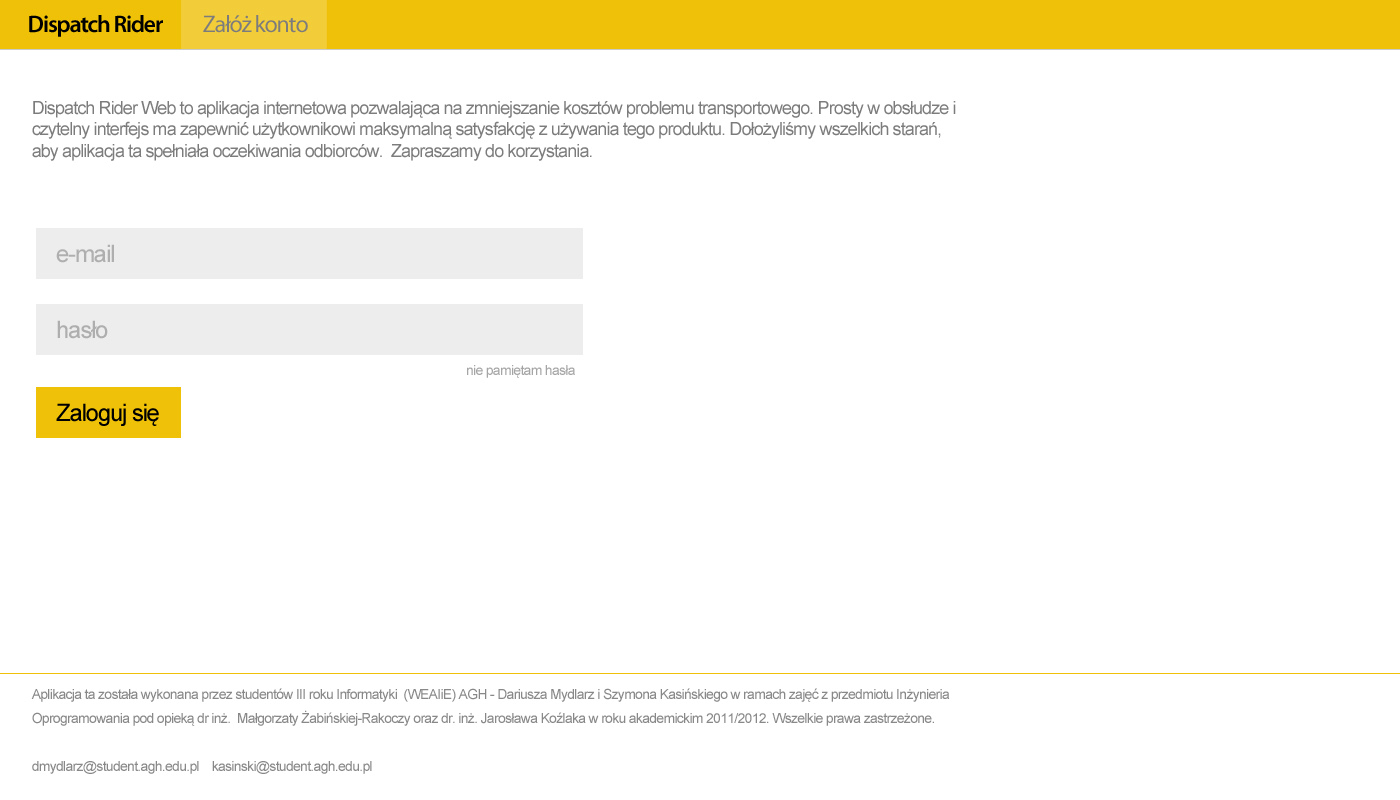
\includegraphics[scale=0.3]{imgs/unlogged_home.jpg}

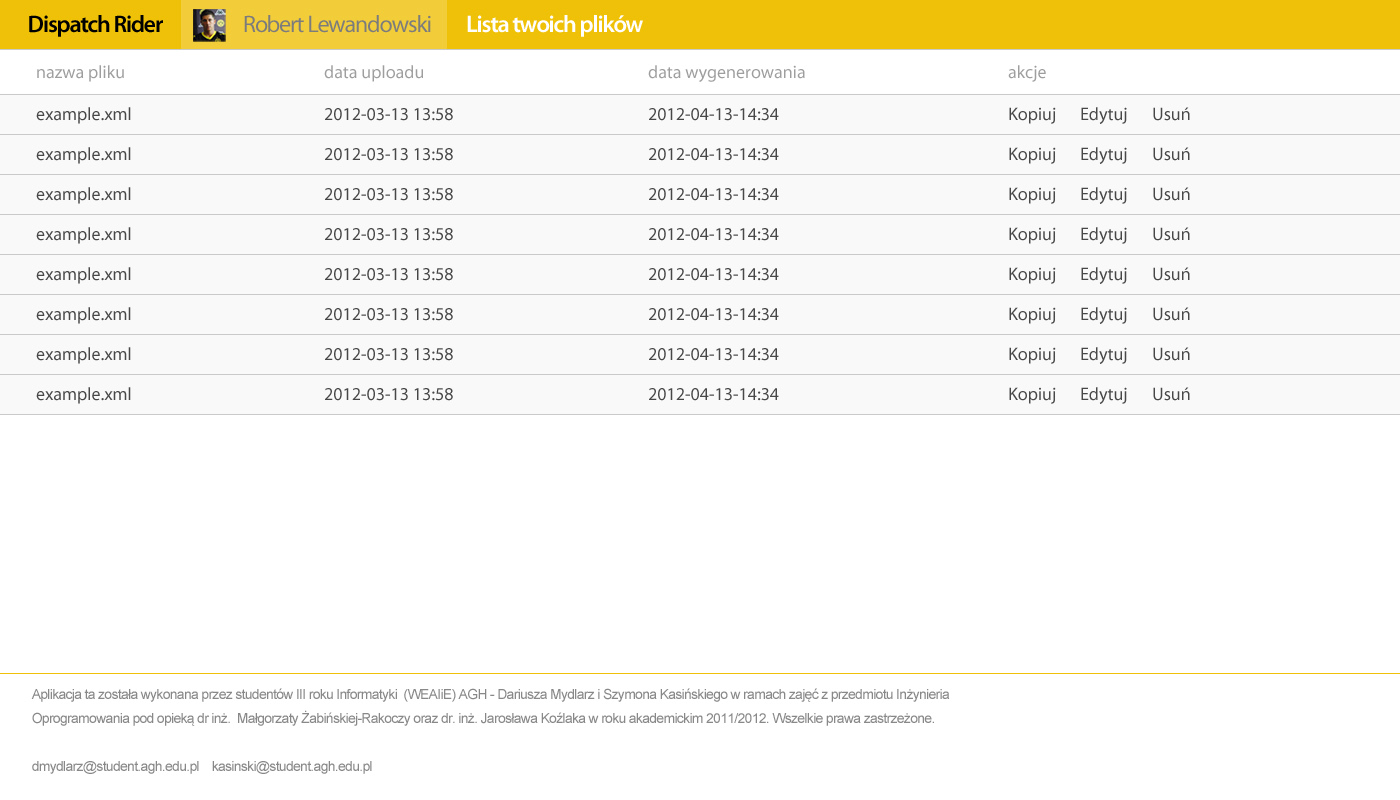
\includegraphics[scale=0.3]{imgs/logged_home.jpg}

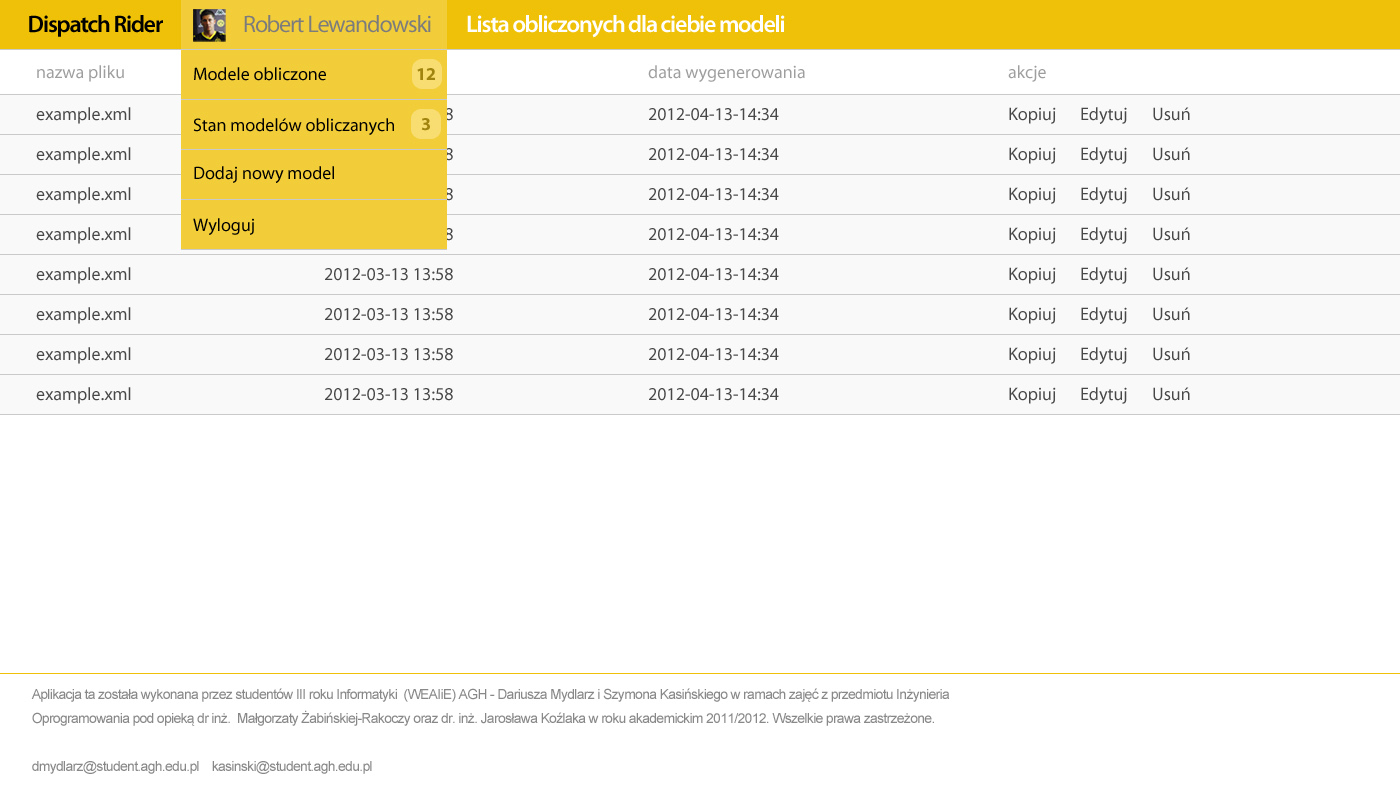
\includegraphics[scale=0.3]{imgs/logged_home_menu.jpg}

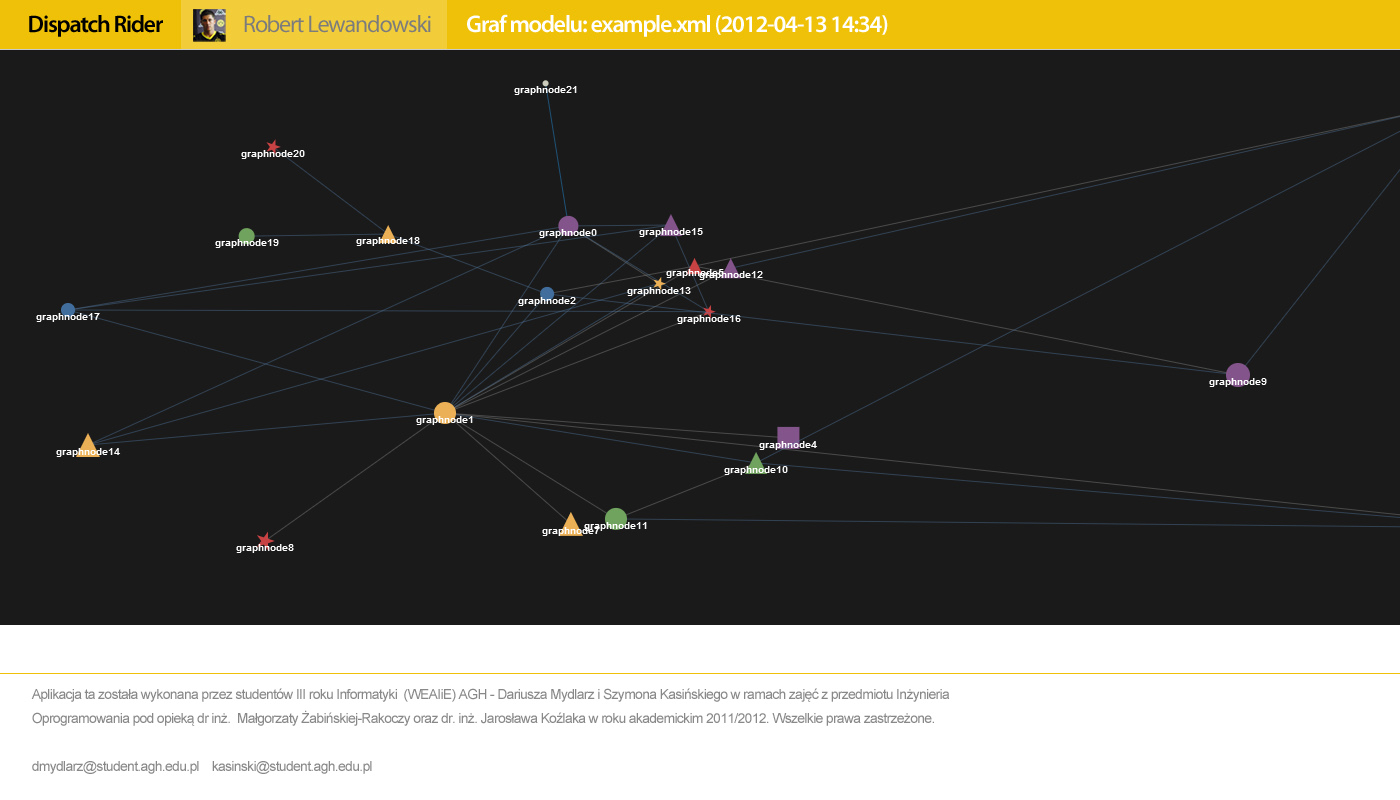
\includegraphics[scale=0.3]{imgs/logged_graph_viewjpg.jpg}
\end{center}

% \chapter{Podział pozostałej do wykonania pracy}
Przechodząc do etapu implementacji systemu podjęliśmy istotne decyzje dotyczące sposobu zaprogramowania systemu. Warstwa prezentacji systemu zostanie zbudowana z użyciem wybranej wcześniej biblioteki służącej do wizualizacji grafów, oraz języka PHP. W założeniu dążymy do zbudowania aplikacji uruchamianej lokalnie z własnym serwerem, jednakże w przyszłości powinna ona zostać rozwinięta o bazę danych oraz funkcjonalności logowania co umożliwi zdalne korzystanie z systemu. 


\textbf{Praca pozostała do wykonania:}

\begin{enumerate}
	\item Stworzenie generatora plików konfiguracyjnych DR. Obsługa wczytania i parsowania plików wgrywanych do systemu - 14.05.2012
	\item Implementacja w systemie pól do prezentacji wyników działania programu w postaci tekstowej - 21.05.2012
	\item Implementacja w systemie funkcjonalności udostępnianych przez bibliotekę prezentacji grafów - 28.05.2012
	\item Integracja i testy systemu - 4.06.2012
\end{enumerate}


\textbf{Praca wykonana:}

\begin{enumerate}
	\item Stworzenie zrębu dokumentacji, uzupełnianej w miarę postępu prac nad systemem.
	\item Stworzenie projektu wyglądu graficznego interfejsu użytkownika.
	\item Implementacja szkieletu systemu, stworzenie layoutu, menu wyboru.
	\item Obsługa kolejkowania zadań oraz uruchamiania systemu DR w miarę nadchodzenia kolejnych zleceń.
\end{enumerate}
\chapter{Architektura systemu}
Architektura budowanego systemu nie będzie skomplikowana. Całość uruchamiana
będzie na jednej maszynie -- serwerze. Całość, to znaczy: aplikacja internetowa, scheduler
oraz Dispatch Rider.
\section{Aplikacja internetowa}
Aplikacja internetowa to miejsce, w którym użytkownik będzie mógł łączyć się z systemem.
Zostanie napisana między innymi przy użyciu języka PHP, co oznacza, że na serwerze,
na którym zostanie uruchomiona aplikacja konieczna będzie jego obsługa.

Najważniejsze z punktu widzenia całego systemu będą znajdujące się w niej 2 katalogi: \texttt{uploads}
oraz \texttt{ready}. W pierwszym będą pojawiać się pliki z właściwościami i konfiguracją wysyłane przez 
użytkownika. Każdy zestaw plików w osobnym folderze o nazwie utworzonej z nazwy wybranej przy uploadzie
przez użytkownika. Pliki te będzie można edytować z poziomu aplikacji www do momentu, aż nie zostaną
przejęte przez schedulera do dalszego przetwarzania. Po zakończeniu przetwarzania problemu przez Dispatch
Ridera, pliki wynikowe wylądują w folderze \texttt{ready}. Aplikacja internetowa będzie przeglądać
każdy z tych katalogów w celu wyświetlenia użytkownikowi informacji na temat przebiegu przetwarzania.

Poza tym w aplikacji internetowej będzie można podejrzeć graf problemu zbudowany w oparciu o pliki
wynikowe z Dispatch Ridera, co jest głównym celem tego projektu. Graf będzie utworzony przy pomocy
biblioteki \texttt{JavaScript InfoVis Toolkit}.

\section{Scheduler}
Scheduler to osobna aplikacji napisana w Javie służąca do kolejkowania zadań przesłanych do systemu
przez użytkownika. Skanuje ona zawartość folderów \texttt{uploads} i \texttt{ready} z aplikacji internetowej
i zarządza ich przesyłaniem do Dispatch Ridera. Scheduler jest więc łącznikiem pomiędzy usługą kliencką,
a serwerową. W momencie ukończenia przetwarzania problemu przez Dispatch Ridera scheduler przenosi pliki
wynikowe do odpowiedniego podfolderu katalogu \texttt{ready} i jeśli jakiś problem czeka już w kolejce
do obliczeń, to przesyła go do Dispatcha.

\section{Dispatch Rider}
Serce całego systemu. Aplikacja, która zajmuje się wykonywaniem wszystkich obliczeń związanych z danym problemem.
Wykorzystana będzie gotowa już aplikacja, napisana przez naszych starszych kolegów, w którą nię będziemy
ingerować, a jedynie skorzystamy z jej plików wynikowych. Aplikacja jest uruchamiana i zarządzana przez schedulera.
\lstset{language=Java}
\chapter{Oprogramowanie schedulera}
W celu obsługi kolejnych zadań przesyłanych do systemu, powstał szkielet oprogramowania zarządzającego kolejkowaniem oraz uruchamianiem Dispatch Ridera z kolejnymi zestawami danych.


Skrypt przeszukuje podany w parametrach startowych katalog systemu plików, poszukując nowo dodanych zestawów danych. W przypadku gdy taki zestaw się pojawia, umieszcza plik 'configuration.xml' zestawu w kolejce zadań do wykonania.


Następnie scheduler sprawdza czy pojawiły się pliki wynikowe działania programu, co jest jednoznaczne z zakończeniem wykonywania danego zadania. Jeśli pliki znajdują się w katalogu wynikowym, wówczas uruchamiane jest kolejne zadanie z kolejki. 


Kwestią istotną jest fakt, iż aby system zadziałał, plik \texttt{configuration.xml} musi znajdować się w katalogu głównym Dispatch Ridera. Ów wymóg jest podyktowany zapewne założeniem projektowym lub błędem DR. W związku z tym, plik ten dla każdego nowo uruchamianego zadania jest kopiowany do głównego katalogu przed uruchomienim procesu. 


Kwestią pozostałą do uzgodnienia pozostaje w tej chwili struktura katalogów tworzona podczas ładowania plików z danymi do systemu - scheduler działa poprawnie, jednak konieczne jest wypracowanie polityki zarządzania danymi wejściowymi. Dyskusję dotyczącą tego zagadnienia przeprowadzimy podczas tworzenia systemu wczytywania i parsowania danych wejściowych.




\subsubsection{Dodane 25.05.2012: Problem z uzyskaniem wyników działania programu}

Jak pisaliśmy powyżej, do uruchomienia Dispatch Ridera wykorzystujemy skrypt napisany w języku Java. Wykonywane jest następujące polecenie systemowe:

\begin{verbatim}
command = "java -cp " + mainPath + "/jar/DTP.jar jade.Boot -nomtp
 TestAgent:dtp.jade.test.TestAgent(" + mainPath +"/configuration.xml)
 InfoAgent:dtp.jade.info.InfoAgent
 DistributorAgent:dtp.jade.distributor.DistributorAgent
 CrisisManagerAgent:dtp.jade.crisismanager.CrisisManagerAgent";
\end{verbatim}

Niestety program uruchamiany w ten sposób - który jest sposobem poprawnym, gdyż powoduje wyświetlenie okna spisu e-unitów oraz wykresu - nie generuje w efekcie żadnych wyników. Pliki które powinny pojawić się w katalogu wyjściowym nie są wogóle tworzone. Problem z całą pewnością leży w sposobie uruchamiania, ponieważ ten sam plik configuration.xml uruchomiony przy pomocy oryginalnego GUI powoduje generowanie wyników. W celu wyjaśnienia tej sytuacji skontaktowaliśmy się z autorami oprogramowania.

\subsubsection{Dodane 14.06.2012: Problemy z uruchomieniem DR przy pomocy Schedulera - ciąg dalszy}

W celu rozwiązania problemów z uruchamianiem DR nawiązaliśmy kontakt z autorem oprogramowania - Sebastianem Pisarskim. Niestety, nie był on w stanie podać rozwiązania naszego problemu ani sposobu uruchamiania DR z linii poleceń systemu (z podaniem ścieżki do pliku configuration.xml). Co więcej, w chwili obecnej nie jesteśmy nawet w stanie uruchomić DR, mimo iż we wcześniejszej wersji ( z marca br. ) było to możliwe.

Podsumowując prace nad oprogramowaniem Schedulera - mimo poprawności stworzonego przez nas kodu, obsługującego operacje na systemie plików, nie udało nam się uruchomić tej funkcjonalności. Przeszkodą nie do pokonania okazało się w tym przypadku uruchomienie oprogramowania DR z linii komend - sposób wykorzystywany przez autorów wcześniej powstałego GUI webowego nie działał, a sam autor Dispatch Ridera nie był w stanie poinformować nas jaki jest poprawny sposób uruchomienia systemu. Również mimo podjętych wielokrotnych prób nie udało nam się doświadczalnie uruchomić programu. Uznajemy że wykorzystaliśmy wszelkie możliwości na poznanie sposobu uruchomienia programu, i bez wypracowania polityki uruchomienia przez autora DR, scheduler nie będzie mógł zadziałać. Problem uruchomienia systemu nie leży po stronie naszego webowego klienta, lecz niestety po stronie samego Dispatch Ridera.
\chapter{Instrukcja obsługi}
\section{Wstęp}
Poniżej przedstawiamy krótką instrukcję obsługi systemu przez nas zbudowanego.
Instrukcja dotyczy części webowej. Niestety nie udało nam się uruchomić schedulera z linii
poleceń, więc nie opisujemy co zrobić by system działał razem z nim.
\\
Do uruchomienia aplikacji webowej potrzebujemy uruchomiony serwer PHP oraz interpreter Pythona.
Całą strukturę katalagów przenosimy do folderu ze stronami naszego serwera PHP (tak, aby móc
się do niego dostać poprzez adres \texttt{http://localhost/nazwa-katalogu}).
\\
Aplikację powinno się uruchamiać w przeglądarce wspierającej HTML5. My testowaliśmy ją w przeglądarce
Google Chrome (v. 19), w której sprawowała się bardzo dobrze.
\\
Jeśli wszystko pójdzie sprawnie powinniśmy ujrzeć ekran powitalny. Po najechaniu myszką w napis
\textbf{Web Dispatch Rider} pojawi nam się menu z trzema pozycjami na liście.

\section{Dodawanie zadania}
W tym widoku użytkownik może dodać nowe zadanie do systemu poprzez zdefiniowanie jego nazwy
oraz wybranie odpowiednich plików dotyczących zadania. System nie pozwoli na wysłanie plików
w niepoprawnym formacie, bądź w sytuacji, w której nie zostaną podane wszystkie pliki
przez użytkownika. W przypadku poprawnego wykonania się operacji przesłania plików
użytkownik otrzyma na ten temat stosowny komunikat, a skrypt Pythonowski utworzy na serwerze
plik w JavaScripcie ze współrzędnymi odzwierciedlającymi mapkę danego zadania.

\section{Zadania w trakcie}
W tym miejscu użytkownik może podejrzeć listę zadań, które czekają w kolejce na bycie przetworzonym
przez zewnętrzny moduł Dispatch Ridera. Do momentu rozpoczęcia przetwarzania użytkownik ma możliwość
edycji tych plików zgodnie z własną wolą. Kiedy system przejmie zadanie, wówczas edycja nie jest już
możliwa.

\section{Zadania obliczone}
Tutaj znajduje się lista zadań gotowych do obejrzenia przez użytkownika. Może on obejrzeć graf dotyczący
danego zadania lub usunąć zadanie. Dane te są dostępne dla użytkownika cały czas. W przypadku gdy
zadanie jest jeszcze liczone, bądź czeka w kolejce użytkownikowi wyświetla się tylko mapka dotycząca danego zadania.

\subsection{Wyświetlanie grafu}
Użytkownik wybierając podgląd grafu danego zadania może zobaczyć jego mapkę oraz przebieg tras wszystkich kierowców.
Mapa pokazuje miejsca z podziałem na miejsca dostarczenia przesyłek i miejsca ich odbioru.
\newline

\begin{center}
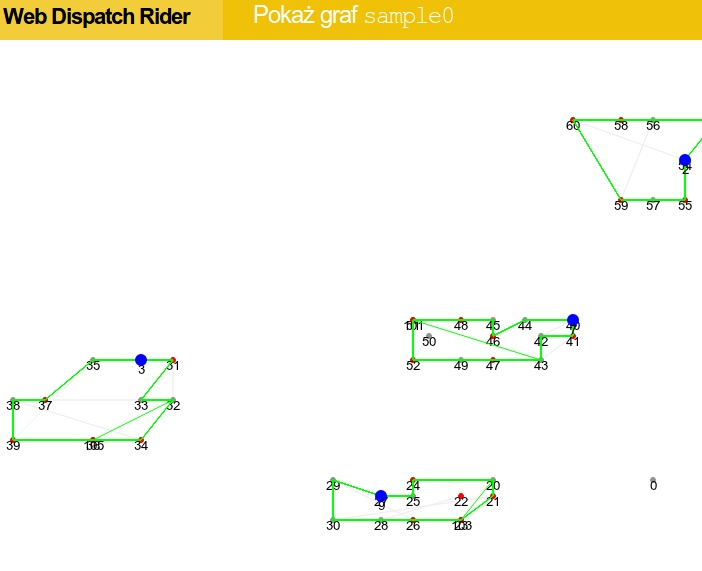
\includegraphics[scale=0.5]{imgs/graf.jpg}
\end{center}

\subsection{Zmiana sposobu wyświetlania grafu}
W dokumentacji należy się również słowo wyjaśnienia odnośnie sposobu wyświetlania grafu.
Na początku semestru uznaliśmy, że skorzystamy z gotowych bibliotek JavaScriptowych analizując je
i wybierając naszym zdaniem najlepszą. Wówczas jednak nie byliśmy do końca świadomi grafu jaki powinniśmy
uzyskać w budowanym przez nas systemie. Biblioteka, którą wybraliśmy nie umożliwiała nam rysowanie grafów/węzłów
w określonych przez nas miejscach ekranu. W związku z tym postanowiliśmy bliżej zaznajomić się z technologią Canvas,
którą dostarcza HTML5. Udało nam się tę znajomość zakończyć pozytywnie i uzyskać poruszający się w przeglądarce graf.
\chapter{Podsumowanie}

W pracy nad interfejsem webowym dla systemu planowania transportu Dispatch Rider odnieśliśmy częściowy sukces. Udało nam się spełnić większość spośród założonych na początku planowania projektu wymagań funkcjonalnych, jednak z przyczyn od nas niezależnych nie byliśmy w stanie uruchomić całej architektury naszej warstwy prezentacji.\\ 
Naszym celem było stworzenie lekkiej, możliwie niezależnej od głównego systemu Dispatch Rider, aplikacji klienckiej służącej do uruchamiania DR oraz prezentowania wyników jego pracy.\\Decyzja o budowie nowej aplikacji klienckiej zamiast rozwijania dotychczas istniejącej była motywowana problemami z uruchomieniem owej już istniejącej wersji webowego gui. Jak wspominaliśmy na początku dokumentacji, nie byliśmy w stanie uruchomić jej na części systemów operacyjnych/przeglądarek, a nawet po uruchomieniu nie była ona w stanie komunikować się z DR.\\
W chwili obecnej, bogatsi o doświadczenia z pracy nad aplikacją, możemy stwierdzić iż wina leżała nie tylko po stronie aplikacji webowej, ale i samego Dispatch Ridera.\\
Program nie posiada wyspecyfikowanych interfejsów umożliwiających komunikację z systemem webowym. W związku z tym, podobnie jak nasi poprzednicy, postanowiliśmy operować na systemie plików, w odpowiedni sposób operując danymi wejściowymi oraz wyjściowymi.
Niestety, nie udało się nam uruchomić z powodzeniem DR z linii poleceń systemu - co jest warunkiem koniecznym w przypadku naszej architektury. Mimo wielokrotnych prób, eksperymentów nie udało nam się wypracować sposobu uruchomienia, co więcej, sam autor systemu nie był w stanie poinformować nas o poprawnym sposobie uruchamiania aplikacji Dispatch Rider. 
\\
Mimo powyższych problemów - które niestety uniemożliwiają nam zaprezentowanie wszystkich funkcjonalności naszej aplikacji - udało nam się spełnić pozostałe zdefiniowane przez nas jako najważniejsze i zaakceptowane przez prowadzących wymagania funkcjonalne. Aplikacja jest w stanie przesyłać oraz wizualizować dane, i może stać się w przyszłości w pełni użyteczna pod warunkiem udostępnienia przez autorów systemu Dispatch Rider interfejsów umożliwiających pewną, skuteczną komunikację z systemem.\\
Możemy uznać że prace zakończyliśmy z sukcesem o tyle, o ile pozwoliły nam na to warunki zewnętrzne. Niestety, sprawdziły się przewidywania poczynione na początku zapoznania z systemem, w których wyrażaliśmy obawy iż sygnalizowane już przez autorów poprzedniej wersji interfejsu webowego problemy z działaniem systemu mogą uniemożliwić działalność części systemu. Za wyjątkowo rozczarowujący uznajemy fakt iż problem sprawiły nam te same kwestie które wymienione były przez autorów wcześniejszej wersji GUI, co oznacza iż nie zostały one naprawione przez rok w którym oprogramowanie DR było ciągle rozwijane.


\section{Analiza spełnienia wymagań funkcjonalnych}

\begin{tabularx}{\textwidth}{ |X|p{2cm}| }
  \hline
  Generowanie pliku określającego zlecenia, o składni: ilość-pojazdów ładowność
prędkość
 & TAK  \\
  \hline
  Generowanie pliku określającego czas nadchodzenia zleceń, o składni: nr-lini czas-zlecenia  & TAK  \\
  \hline
  Generowanie pliku zawierającego liczbę kierowców & TAK \\
  \hline
  Generowanie pliku określającego parametry ciągników, o składni: moc niezawodność wygoda zużycie-paliwa typ-zaczepu & TAK \\
  \hline
  Generowanie pliku opisującego parametry naczep o składni: masa pojemność
typ-ładunku uniwersalność typ-zaczepu & TAK \\
  \hline
  Generowanie pliku opisującego parametry holonów o składni: initialCapacity =
pojemność-pojazdu mode = tryb bases = ilość-baz eUnitsCount = ilość-jednostek & TAK \\
  \hline
  Generowanie pliku konfiguracyjnego configuration.xml & TAK \\
  \hline
  Kolejkowanie zadań zlecanych systemowi & NIE \\
  \hline
  Uruchamianie systemu Dispatch Rider z użyciem dostarczonych z zewnątrz lub wygenerowanych plików & NIE \\
  \hline
  Wizualizacja grafu sieci transportowej & TAK \\
  \hline
  Wizualizacja tras pokonanych przez pojazdy & TAK \\
  \hline
  Wyświetlanie informacji o każdym z holonów & TAK \\
  \hline
  Przechowywanie wyników obliczeń, w celu zaprezentowania na żądanie & TAK \\
  \hline
\end{tabularx}
\\ \\
Jak więc widać z powyższej tabeli większość funkcjonalności udało nam się uzyskać. Te, które się nie powiodły
wynikły z problemów związanych z dostarczonym systemem Dispatch Rider, bądź złym rozplanowaniem czasu wykonania
projektu. Mimo wszystko, najważniejsze wymagania, takie jak ładowanie zadań do systemu oraz wizualizacja tras
jak najbardziej udało nam się uzyskać, dzięki czemu oceniamy projekt jako zakończony sukcesem.

\section{Napotkane błędy systemu DispatchRider}
\begin{itemize}
	\item System nie uruchamia się wogóle przy pomocy linii poleceń w przypadku gdy plik 'configuration.xml' znajduje się gdzie indziej niż katalog główny programu. Nie mają na to wpływu zawarte w nim ścieżki względne, gdyż nawet po zamianie ich na bezwzględne, plik ten musi zostać skopiowany do katalogu głównego by móc go uruchomić.
	\item Brak generowania pliku wynikowego. W trakcie prac na Schedulerem napotkaliśmy na (wspomnianą już przez zespół Baran-Patrzyk) sytuację gdy Dispatch Rider nie generował plików wynikowych nawet wówczas gdy udawało nam się uruchomić system. Problem ten w efekcie uniemożliwił nam zrealizowanie wszystkich funkcjonalności systemu.
	\item Problem uruchomienia GUI wbudowanego w Dispatch Riderze. Do pewnego momentu prac, udawało nam się uruchamiać Dispatch Ridera za pomocą komendy \textbf{java -jar GUI.jar}. Niestety, w kolejnej wersji systemu funkcjonalność ta przestała działać, i otrzymywalismy  (na obydwu stacjach roboczych) błąd \textbf{Problem with reading file:xmlschemes/configuration.xsd (No such file or directory) }. Autor systemu nie był w stanie nam pomóc, stwierdzając że u niego dana funkcjonalność działa.
\end{itemize}
\begin{thebibliography}{2}
\bibitem{holony} 
  Gołacki M.:
  \emph{Modelowanie Transportu z użyciem Holonów}. Kraków, wrzesień 2009.
\bibitem{sytuacje-kryzysowe} 
  Konieczny M.:
  \emph{Modelowanie i optymalizacja transportu w sytuacjach kryzysowych}. Kraków, 2008.
\bibitem{podejscie-holoniczna} 
  Miąsko T., Pisarski S..:
  \emph{Dispatch Rider. Podejście holoniczne w problemie transportowym}. Dokumentacja projektu KI AGH 2010.
  
\end{thebibliography}



\end{document}
